\documentclass[tikz,border=8pt]{standalone}
\usepackage{pgfplots}
\pgfplotsset{compat=1.18}
\definecolor{chapterteal}{HTML}{196F6B}
\definecolor{chapterrust}{HTML}{A3472F}
\definecolor{chaptergold}{HTML}{C58B18}
\definecolor{chapterblue}{HTML}{174F75}

\begin{document}

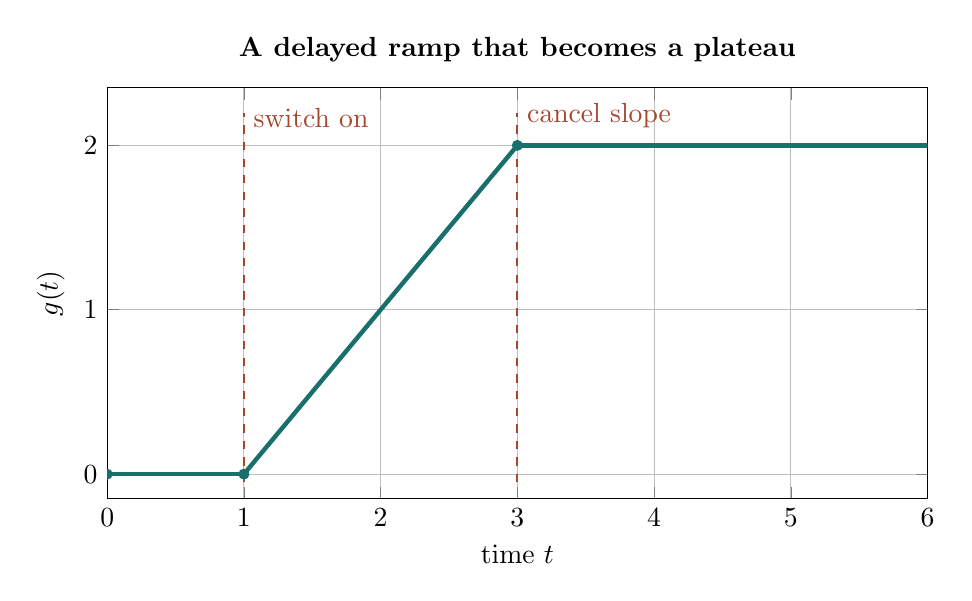
\begin{tikzpicture}
\begin{axis}[
  width=12cm,
  height=6.8cm,
  xmin=0,xmax=6,
  ymin=-0.15,ymax=2.35,
  xlabel={time $t$},
  ylabel={$g(t)$},
  title={A delayed ramp that becomes a plateau},
  title style={font=\bfseries},
  grid=both,
  xtick={0,1,2,3,4,5,6},
  ytick={0,1,2}
]
\addplot[chapterteal,ultra thick] coordinates {(0,0) (1,0)};
\addplot[chapterteal,ultra thick] coordinates {(1,0) (3,2)};
\addplot[chapterteal,ultra thick] coordinates {(3,2) (6,2)};
\addplot[chapterrust,dashed,thick] coordinates {(1,-0.05) (1,2.2)};
\addplot[chapterrust,dashed,thick] coordinates {(3,-0.05) (3,2.2)};
\node[chapterrust,anchor=south west] at (axis cs:1,2.05) {switch on};
\node[chapterrust,anchor=south west] at (axis cs:3,2.05) {cancel slope};
\fill[chapterteal] (axis cs:0,0) circle (2pt);
\fill[chapterteal] (axis cs:1,0) circle (2pt);
\fill[chapterteal] (axis cs:3,2) circle (2pt);
\end{axis}
\end{tikzpicture}

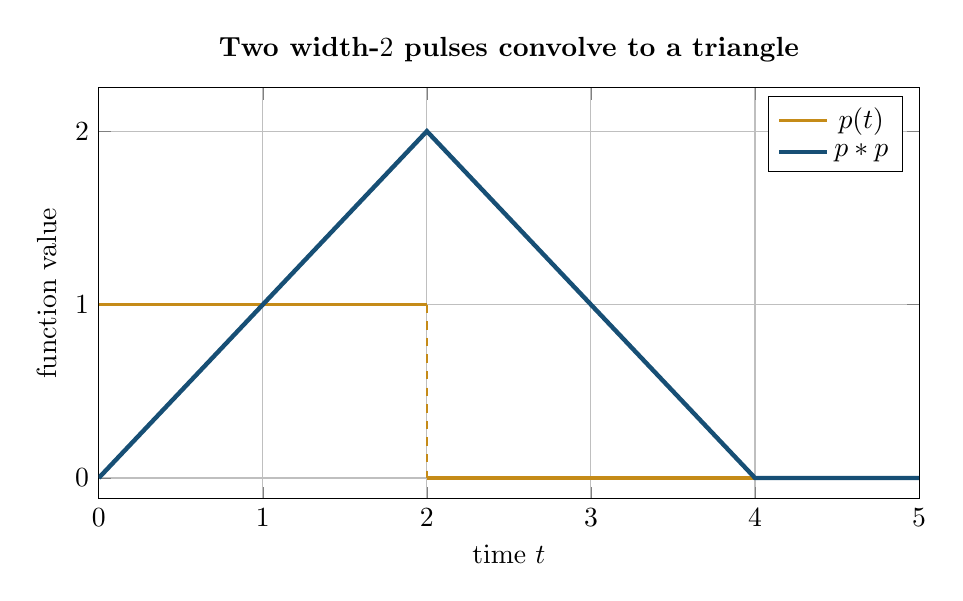
\begin{tikzpicture}
\begin{axis}[
  width=12cm,
  height=6.8cm,
  xmin=0,xmax=5,
  ymin=-0.12,ymax=2.25,
  xlabel={time $t$},
  ylabel={function value},
  title={Two width-$2$ pulses convolve to a triangle},
  title style={font=\bfseries},
  grid=both,
  xtick={0,1,2,3,4,5},
  ytick={0,1,2},
  legend style={at={(0.98,0.98)},anchor=north east}
]
\addplot[chaptergold,very thick] coordinates {(0,1) (2,1)};
\addlegendentry{$p(t)$}
\addplot[chaptergold,dashed,thick,forget plot] coordinates {(2,1) (2,0)};
\addplot[chaptergold,very thick,forget plot] coordinates {(2,0) (5,0)};
\addplot[chapterblue,ultra thick] coordinates {(0,0) (2,2) (4,0) (5,0)};
\addlegendentry{$p*p$}
\end{axis}
\end{tikzpicture}

\end{document}
